\chapter{Evaluierung der erstellten Modelle} % (fold)
\label{cha:eval_modell}

Im zweiten Teil der Evaluierung wird nicht der Umgang mit dem Werkzeug betrachtet (siehe dazu Kapitel \ref{cha:eval_werkzeug}), sondern auf das unmittelbare Resultat der Werkzeugverwendung, also das erstellte Modell eingegangen. Ebenfalls nicht Gegenstand der Untersuchung ist in diesem Abschnitt die Wirkung der Modellbildung auf die operative Arbeit („Production Work“), die in Kapitel \ref{cha:eval_aw} betrachtet wird.

Ausgehend von den erstellten Modellen und deren Entstehungsprozess wird also in diesem Kapitel untersucht, wie das Werkzeug auf die in dieser Arbeit gewählte Form der Unterstützung expliziter „Articulation Work“, nämliche der kooperativen Externalisierung und Abstimmung mentaler Modelle, wirkt. Dementsprechend sind die im folgenden Abschnitt beschrieben Hypothesen aus den Ausführungen der Kapitel über mentale Modelle (Kapitel \ref{cha:mentale_modelle}) und der Methodik zur Externalisierung derselben (Kapitel \ref{cha:methodik}) abgeleitet. 

Zusätzlich wird eine explorativ gebildete Hypothese untersucht, die sich auf inhaltlicher Ebene mit dem Phänomen der Abbildung von Zusammenhängen durch räumliche Konfiguration der Konzepte in einem Modell beschäftigt, das in der Untersuchung der Hypothese \ref{hyp:diagmodelle} bereits hinsichtlich der Werkzeugverwendung beschrieben wurde.

\section{Hypothesen} % (fold)
\label{sec:m_hypothesen}

In diesem Abschnitt werden die Hypothesen abgeleitet, die in diesem Kapitel geprüft werden. Wie in Kapitel \ref{cha:eval_werkzeug} ist zwischen konzeptuell aus der Aufgabenstellung bzw. der entwickelten Methodik abgeleiteten Hypothesen über die Wirkung des Werkzeugs und explorativ während der Evaluierung selbst gebildeten Hypothesen über Eigenschaften des Werkzeugs bzw. dessen Verwendung im Kontext der Modellbildung zu unterscheiden.

\subsection{Konzeptuell begründete Hypothesen} % (fold)
\label{sub:m_konzeptionell_begründete_hypothesen}

Die folgenden Hypothesen sind aus der Aufgabenstellung bzw. den Ausführungen zur Modellierungs-Methodik abgeleitet. Auf die entsprechenden Ausführungen in den Kapiteln \ref{cha:mentale_modelle} bzw. \ref{cha:methodik} wird jeweils bei der Begründung der Hypothesen verwiesen.

Ein wesentlicher Aspekt bei der Externalisierung mentaler Modelle ist die Offenheit der Repräsentationssprache. Diese ist aus Abschnitt \ref{sub:concept_mapping} begründbar und in Anforderung \ref{anf:nicht_vorgegebene_semantik_der_modellierungselemente} abgebildet. Unter „Offenheit“ ist in diesem Zusammenhang die Eigenschaft der Repräsentationssprache gemeint, keine vordefinierte Semantik der Modellelemente vorzugeben sondern diese von den Modellierenden festlegen zu lassen. Dies umfasst im vorliegenden Fall sowohl die Bedeutung der unterschiedlichen Konzepttypen als auch die Bedeutung der Verbindungen zwischen Konzepten. Das Werkzeug darf also in diesem Zusammenhang die Benutzer nicht bei der Wahl der Repräsentationskonzepte und damit bei der Externalisierung selbst einschränken.

\begin{hyp}
	\label{hyp:keine_einschränkung}
	Das Werkzeug schränkt Benutzer semantisch nicht bei der Externalisierung ihrer mentalen Modelle ein.
\end{hyp}

Das Argument der Nicht-Beschränkung der Benutzer bei der Externalisierung hat neben der eben beschriebenen Sprach-Dimension auch eine konkrete Modell-Dimension. Während sich obige Hypothese auf semantische Einschränkungen der Externalisieungsmöglichkeiten bezieht, ist sind auch konkrete, strukturelle Einschränkungen bei der Verwendung des Werkzeugs zur Externalisierung eines bestimmten mentalen Modells zu berücksichtigten. Die Externalisierung muss -- um nicht beschränkend zu wirken -- beliebig umfangreiche Modelle ermöglichen. „Umfangreich“ bedeutet hier, dass das Modell beliebig viele Elemente enthalten können muss und diese beliebig untereinander in Beziehung gesetzt werden können.
	
\begin{hyp}
	\label{hyp:beliebige_komplexität}
	Das Werkzeug ermöglicht die Repräsentation beliebig umfangreicher Modelle.
\end{hyp}

Die Externalisierung mentaler Modelle mit Hilfe von computer-gestützten Werkzeugen ist keine originäre Idee dieser Arbeit. Computerunterstützung existiert vor allem im Bereich des „Concept Mapping“ (siehe Abschnitt \ref{sub:concept_mapping}), das methodisch maßgeblich in das vorgeschlagene Vorgehen des hier vorgestellten Ansatzes einfließt (siehe Kapitel \ref{cha:methodik}). In den existierenden Werkzeugen werden jedoch die kooperative Erstellung und kommunikative Validierung der externalisierten Modelle nicht explizit berücksichtigt. Beide Aspekte sind jedoch -- wie bei der Beschreibung der Strukturlegetechniken \ref{sub:strukturlegetechniken} ausgeführt -- wichtig für den Abgleich mentaler Modelle und damit für die erfolgreiche Durchführung von „Articulation Work“. Die Ermöglichung und Stärkung der Kooperation der Beteiligten untereinander ist also ein wesentlicher Teilaspekt der Anforderung \ref{anf:kollaborative_und_unmittelbare_manipulierbarkeit_des_modells} an das Werkzeug („Kooperative und unmittelbare Manipulierbarkeit des Modells“).

\begin{hyp}
	\label{hyp:stärkere_kooperation}
	Die Verwendung des Werkzeugs führt zu stärkerer Kooperation bei der Modellerstellung als die Verwendung von bildschirm-basierten Werkzeugen.
\end{hyp}

% subsection konzeptionell_begründete_hypothesen (end)

\subsection{Explorativ gebildete Hypothesen} % (fold)
\label{sub:m_explorativ_gebildete_hypothesen}

Im Verlauf der beiden Evaluationen war die Herstellung von Verbindungen zwischen Modellelementen aus technischen Gründen schwierig zu benutzen und sehr anfällig für Fehlfunktionen. Dies führte dazu, dass Verbinder nahezu nicht verwendet wurden (siehe dazu die Auswertungen zu Hypothese \ref{hyp:diagmodelle} in Abschnitt \ref{sub:repräsentation_diagrammatischer_modelle}). In dieser Situation wurden Beziehungen zwischen Modellelementen von den Benutzern durch die räumliche Anordnung der Elemente ausgedrückt. Diese implizite Darstellung von relationaler Information erfolgte in allen Fällen spontan und ohne Anleitung oder Instruktion. Dies führte zu der Vermutung, dass die Verwendung von Verbindern zur Abbildung von Beziehungen bzw. Zusammenhängen zwischen Elementen nicht notwendig ist. Um diese Vermutung zu prüfen, wurde sie formal als Hypothese \ref{hyp:keine_verbinder} in die Untersuchung aufgenommen.

\begin{hyp}
	\label{hyp:keine_verbinder}
	Zur Abbildung von Zusammenhängen ist die Verwendung von Verbindern nicht notwendig.
\end{hyp}

% subsection explorativ_gebildete_hypothesen (end)

% section hypothesen (end)

\section{Untersuchungsdesign und Durchführung} % (fold)
\label{sec:m_untersuchungsdesign}

In diesem Abschnitt wird auf Basis der oben formulierten Hypothesen das Untersuchungsdesign abgeleitet und die Durchführung der Untersuchung beschrieben. Der erste Teil des Abschnitts beschreibt die Operationalisierung der Hypothesen und damit die Festlegung wie diese konkret geprüft werden können. Im zweiten Teil des Abschnitts wird die Durchführung der Prüfung beschrieben. Hier erfolgt neben der Zuordnung der einzelnen Modellierungsblöcke (siehe Abschnitt \ref{sec:globales_untersuchungsdesign}) auch die Darstellung rein beschreibender Modell-Parameter, die nicht unmittelbar in die Prüfung der Hypothesen eingehen. 

\subsection{Operationalisierung} % (fold)
\label{sub:m_operationalisierung}

In diesem Abschnitt wird für jede Hypothese identifiziert, in welcher Form sie geprüft werden kann. Dies umfasst die Festlegung der Messpunkte sowie der jeweiligen Mess- und Auswertungsmethode (letzte bezugnehmend auf den in Abschnitt \ref{sec:eingesetzte_werkzeuge_und_verfahren} beschriebenen Verfahren). Zudem werden jene Evaluationsblöcke festgelegt, die für die jeweilige Untersuchung herangezogen wurden.

Für jede Hypothese wird also spezifiziert, anhand welcher Aspekte diese geprüft werden kann (= abhängige Variablen). Zudem wird festgelegt welche Ausgangssituation bei der Anwendung gewählt werden muss, um die Prüfung durchführen zu können (= unabhängige Variable) und welche Faktoren die Beurteilung ggf. ungewollt beeinflussen können (= Störvariablen).

\subsubsection{Keine semantische Einschränkung der Externalisierung} % (fold)
\label{ssub:keine_semantische_einschränkung_der_externalisierung}

Gegenstand dieses Abschnitts ist die Prüfung der Hypothese \ref{hyp:keine_einschränkung}. Diese bezieht sich auf die geforderte Eigenschaft des Werkzeugs, die Benutzer bei der Modellierung semantisch nicht einzuschränken.

Voraussetzung für die Prüfung dieser Hypothese ist die Verwendung des Werkzeugs zur Modellbildung bei einer Aufgabe, die die semantischen Kategorien der Strukturierung nicht vorgibt. In der eingesetzten Methodik wird die Festlegung von Elementtypen explizit gefordert (Vorgehen und Zeitpunkt dafür werden jedoch nicht vorgegeben). Etwaige Modellierungsvorkenntnisse können diese Festlegung insofern beeinflussen, als dass die Konzepte bekannter Sprachen bevorzugt eingesetzt werden könnten. Im Sinne der Hypothese ist dies jedoch keine Störvariable, da die Forderung nach nicht einschränkender Struktur auch die Verwendung existierender Modellierungssprachen umfassen muss.

Die nicht einschränkende Wirkung kann qualitativ anhand von Benutzeraussagen und dem Prozess und Ergebnis der Modellentstehung beurteilt werden. Im ersten Fall bieten sich neben der direkten Frage nach der Abbildbarkeit der gewünschten Information auch Teilaspekte des \gls{PMS}-Framework \citep{Sedera02} an, das unter anderem die subjektiv wahrgenommene Qualität des Modellierungsergebnisses und die Abbildbarkeit der subjektiv wichtigen Information im Modell abbildet (zur Eignung des \gls{PMS}-Frameworks im Kontext dieser Arbeit siehe \citep{Wahlmuller10}). Am Prozess- und Ergebnis der Modellentstehung selbst kann beurteilt werden, ob und inwieweit die zur Verfügung gestellten, semantisch nicht vorbelegten Modellierungselemente für die Abbildung der gewünschten Information ausreichend bzw. geeignet waren. Dazu kann betrachtet werden, ob die beschränkte Anzahl von Elementen im Verlauf der Modellierung zu verändertem Vorgehen in der Abbildung oder zur Nichtabbildung bestimmter Modellaspekte führte und ob durch semantische Mehrfachbelegung bzw. die Einführung von nicht als Modellierungselement vorgesehenen Bausteinen der Sprachumfang über das ursprünglich intendierte Maß hinaus erweitert wurde. 

Vergleichend können zusätzlich Modelle herangezogen werden, die aus identischen Fragestellungen wie jene mit dem Werkzeug erstellten resultieren, bei denen jedoch ein in der Anzahl und Semantik der Modellierungselemente frei erweiterbares Werkzeug zum Einsatz kommt. Hier ist von Interesse, ob die erstellten Modelle semantisch vielfältiger sind als jene, die mit dem hier vorgestellten Werkzeug erstellt wurden.

% subsubsection keine_semantische_einschränkung_der_externalisierung (end)

\subsubsection{Repräsentation beliebig umfangreicher Modelle} % (fold)
\label{ssub:repräsentation_beliebig_komplexer_modelle}

Gegenstand dieses Abschnitts ist die Operationalisierung der Hypothese \ref{hyp:beliebige_komplexität}. Dabei wird überprüft, ob das Werkzeug die Abbildung beliebig umfangreicher Modellierungsaufgaben ermöglicht.

Voraussetzung zur Prüfung dieser Hypothese ist die Verwendung von Modellierungsaufgaben, die zu umfangreichen Modellen führen. Umfangreichen Modellierungsaufgaben sind Aufgaben, die bei detaillierter Modellierung >15 Modellelemente benötigen\footnote{15 wurde als Grenze gewählt, weil diese Anzahl die Obergrenze an gleichzeitig am Werkzeug verwendbaren Elementen darstellt}). Dies ist deshalb notwendig, weil der wesentliche beschränkende Faktor des Umfangs eines Modells am hier vorgestellten Werkzeug die physisch eingeschränkte Größe der Modellierungsoberfläche ist. Etwaige Modellierungsvorkenntnisse der Benutzer sind bei der Prüfung dieser Hypothese nicht von Relevanz.

Um Schlussfolgerungen auf eine etwaig einschränkende Wirkung des Werkzeugs auf den Umfang der Modelle treffen zu können, muss eine entsprechende Aufgabenstellung einerseits mittels dem hier vorgestellten Werkzeug („Experimentalgruppe“) und andererseits mit einem Werkzeug, dass den Umfang der Modellierungsoberfläche nicht begrenzt („Kontrollgruppe“), abgebildet werden. Die Ergebnisse der beiden Gruppen werden dann gegenübergestellt. Falls bei identischer Fragestellung der Umfang der Modelle in der Kontrollgruppe signifikant höher ist als jener der Experimentalgruppe, kann von einer einschränkenden Wirkung ausgegangen werden und die Hypothese müsste abgelehnt werden.

Daneben sind wiederum Aussagen der Benutzer über die Abbildbarkeit umfangreicher Modelle zur Prüfung der Hypothese heranzuziehen. Entsprechende Fragen wurden in den Modellierungsblöcken 2, 3, 4 und 5 gestellt, wobei die Fragestellungen in den Blöcken 2 und teilweise 4 eher zu nicht umfangreichen Modellen führte, die auf der Oberfläche ausreichend Platz fanden und deshalb hier nicht berücksichtigt werden können.

% subsubsection repräsentation_beliebig_komplexer_modelle (end)

\subsubsection{Wirkung auf die Kooperation bei der Modellerstellung} % (fold)
\label{ssub:wirkung_auf_die_kooperation_bei_der_modellerstellung}

Gegenstand dieses Abschnitts ist die Operationalisierung der Hypothese \ref{hyp:stärkere_kooperation}. Gegenstand der Untersuchung ist hier, ob die Verwendung des Werkzeugs bei der Modellbildung zu stärkerer Kooperation zwischen den Beteiligten führt als der Einsatz von bildschirmbasierten Werkzeugen.

Die Prüfung der Wirkung des Werkzeugs auf die kooperative Abbildung von Modellen bedingt Fragestellungen, die Kooperation explizit einfordern. Etwaige Modellierungsvorkenntnisse beeinflussen die Prüfung der Hypothese nicht. Bei der Beurteilung zu berücksichtigen sind etwaige bestehende persönliche Bekanntschaften oder etablierte Gruppen, deren Zusammenarbeit bereits institutionalisiert ist. Um den Einfluss derartiger Faktoren möglichst auszuschließen, müssen die Gruppen bei der Modellbildung zufällig gebildet werden und etwaige Bekanntschaften innerhalb der gebildeten Gruppen explizit im Vorfeld der Untersuchung erhoben werden.

Die hier zu prüfende Hypothese baut auf Hypothese \ref{hyp:kollaborativ} auf. Dort war zu prüfen, ob das Werkzeug kooperatives Arbeiten grundsätzlich ermöglicht. In diesem Abschnitt wird geprüft, ob der Einsatz des Werkzeugs hinsichtlich der Kooperation der Beteiligten tatsächlich einen meßbaren Vorteil gegenüber einem traditionellen, bildschirmbasierten Werkzeug hat. Dazu ist es notwendig, eine vergleichende Untersuchung durchzuführen. Modellierungsblock 5 wurde dementspechend geplant und umfasste eine die kooperative Abbildung eines Modells sowohl am Modellierungstisch als auch mittels dem bildschirmbasierten Werkzeug CMapTools. Die Aufgabenstellung wurde so gewählt, dass das resultierende Modell grundsätzlich in beiden Werkzeugen abgebildet werden konnte. Untersucht wurde, in welchem Ausmaß Kooperation zwischen den beteiligten Personen auftrat. Als Metriken dienten dazu die Zeitverteilung der Beteiligung am Modellierungsvorgang, der Zeitanteil an Diskussion während der Modellbildung sowie die Anzahl der Initiativwechsel (Turn-taking) während eines Durchgangs.

% subsubsection wirkung_auf_die_kooperation_bei_der_modellerstellung (end)

\subsubsection{Abbildung von Zusammenhängen ohne Verbinder} % (fold)
\label{ssub:abbildung_von_zusammenhängen_ohne_verbinder}

Gegenstand dieses Abschnitts ist die Operationalisierung der Hypothese \ref{hyp:keine_verbinder}. Gegenstand der Untersuchung ist die Beobachtung, dass zur Abbildung von Zusammenhängen die Verwendung von explizit dargestellten Verbindern nicht notwendig ist.

Die Prüfung dieser Hypothese stellt keine Vorbedingungen an die Modellierungsaufgabe oder die Modellierungsvorkenntnisse der Benutzer. Auch können individuelle Anwendungen der Werkzeugs (d.h. nicht nur in kooperativen Szenarien) zur Untersuchung verwendet werden. 

Bei der Prüfung der Hypothese sind zwei Formen der Notwendigkeit von explizit dargestellten Verbindern zu unterscheiden. Zum Einen ist die Notwendigkeit bei der kooperativen Erstellung eines Modells zu untersuchen, bei der sämtliche Beteiligte zu einer einheitlichen Interpretation des dargestellten Modells kommen sollen. Zum Anderen muss auch der Fall einer zeitlich nachgelagerten Interpretation durch Dritte untersucht werden. Hier ist zu erheben, ob die Interpretation der Modellinhalts dem ursprünglichen Verständnis des bzw. der Modellierenden entspricht.

Zur Untersuchung muss dem ursprünglichen Modellierer jeweils eine inhaltliche Interpretation des Modellierungsergebnisses rückgespiegelt werden. Diese Form der kommunikativen Validierung kommt methodisch im Rahmen der Anwendung von Strukturlegetechniken (siehe Abschnitt \ref{sub:strukturlegetechniken}) zum Einsatz und ist deshalb ohnehin Teil der in dieser Arbeit vorgeschlagenen Methodik bei der kooperativen Anwendung des Werkzeugs. Zur zeitlich nachgelagerten Interpretation bedarf es einem separaten Schritt, in dem das Modellierungsergebnis von einer dritten, den der Modellierung nicht beteiligten Person interpretiert und rückgespiegelt wird. 

% subsubsection abbildung_von_zusammenhängen_ohne_verbinder (end)
% subsection m_operationalisierung (end)

\subsection{Durchführung} % (fold)
\label{sub:m_durchführung}

In diesem Abschnitt werden die für diesen Evaluierungs-Teil relevanten deskriptiven Parameter der berücksichtigten Anwendungs-Blöcke angeführt.
Als Grundlage der Überprüfung der Hypothesen werden hier die Evaluierungs-Blöcke 1 bis 5 verwendet. Dabei wurden für die quantitativ zu prüfenden Variablen die Blöcke 2 und 3 herangezogen, da in diesen die größten Stichproben zur Verfügung standen. In die qualitative Auswertung der Ergebnisse wurden hingegen alle Blöcke (1-5) mit einbezogen.

\subsubsection{Stichprobe} % (fold)
\label{ssub:stichprobe}

\begin{tabular}{| p{2cm} || p{2,5cm} | p{2,5cm} | p{2,5cm} || p{2cm} |}
  \hline
   & Aushandlung (1. Durchgang) & Aushandlung (2. Durchgang) & Concept Mapping & Gesamt \\ \hline
   $n_{Anwendungen}$ & 9 & 9 & 17 & 35 \\ 
   $n_{Teilnehmende}$ & 19 & 18 & 47 & 84 \\ \hline
\end{tabular} 

% subsubsection stichprobe (end)

\subsubsection{Modellgröße} % (fold)
\label{ssub:modellgröße}

Die Verteilung der Modellgröße wurde hier anhand der Anzahl der verwendeten Elemente (siehe Abbildung \ref{fig:img_Evaluierung_elementUsageBlocksOverview}) und der Anzahl der verwendeten Verbindungen (siehe Abbildung \ref{fig:img_Evaluierung_elementUsageConnectorsOverview}) dargestellt. Berücksichtigt wurden dabei die Ergebnisse der Modellierungsblöcke 2 („Aushandlung“) und 3 („Concept Mapping“). Die Modelle der Modellierungsblöcke 1 und 4 sind aufgrund der uneinheitlichen Aufgabenstellungen nicht vergleichbar, jener Teil des Modellierungsblocks 5, der mit dem hier vorgestellten Werkzeug durchgeführt wurden, weißt ob der identischen Aufgabenstellung hohe Ähnlichkeit mit den Ergebnissen von Block 3 auf.

\begin{figure}[htbp]
	\centering
		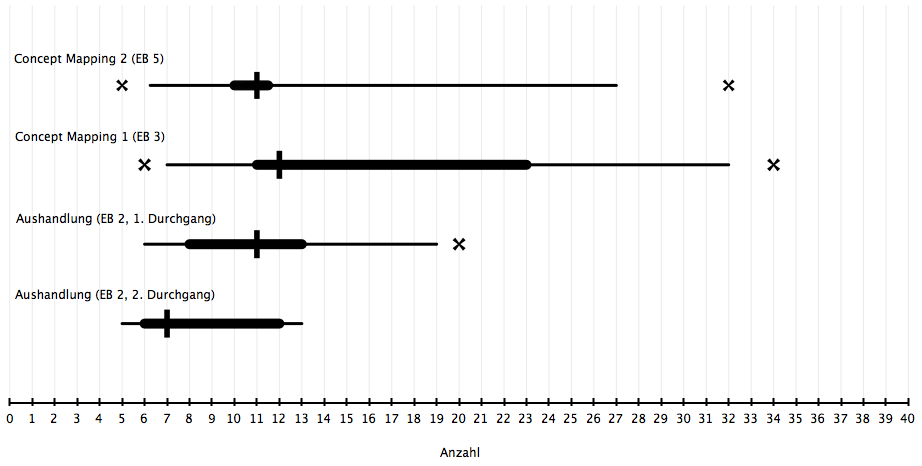
\includegraphics[width=15cm]{img/Evaluierung/elementUsageBlocksOverview.png}
	\caption{Anzahl der verwendeten Elemente -- Übersicht}
	\label{fig:img_Evaluierung_elementUsageBlocksOverview}
\end{figure}

In Abbildung \ref{fig:img_Evaluierung_elementUsageBlocksOverview} ist zu erkennen, dass der Median der Anzahl der verwendeten Elemente zwischen 7 und 12 liegt, wobei die Concept Mapping Aufgabe wegen des nicht explizit vorgegebenen Detaillierungsgrad der Modellierung eine höhere Schwankungsbreite (mit starker Tendenz zu größeren Modellen) aufweist. Zwar war der Detaillierungsgrad der Aushandlungsaufgaben ebenfalls nicht explizit vorgegeben, hier scheint jedoch eine höhere Überstimmung hinsichlich des angemessenen Detaillierungsgrades gegeben gewesen zu sein. 

Auffällig ist außerdem, dass zwischen den beiden Durchgängen des Aushandlungs-Blocks ein (statistisch allerdings wegen der geringen Stichprobengröße nicht signifikanter ($t=0.16 < t(0.95,8)=2.306$)) Unterschied in der Größe der Modelle (gemessen an der Anzahl der Elemente) gegeben ist. Dies scheint nach Betrachtung der qualitativ erhobenen Daten aus den entsprechenden Videoaufzeichnungen einerseits darauf zurückzuführen zu sein, dass der zweite Durchgang in einer späteren Phase des produktiven Arbeitsprozesses durchgeführt wurde, in dem weniger offene Schritte zu behandeln waren, andererseits scheint durch die bereits etablierte Zusammenarbeitsprozesse generell weniger Abstimmungsbedarf gegeben gewesen zu sein. Dieser Eindruck wird auch durch die generell geringere Modellierungdauer in Durchgang 2 (siehe Abbildung \ref{fig:img_Evaluierung_usageTimeNegotiation}) bestärkt.

\begin{figure}[htbp]
	\centering
		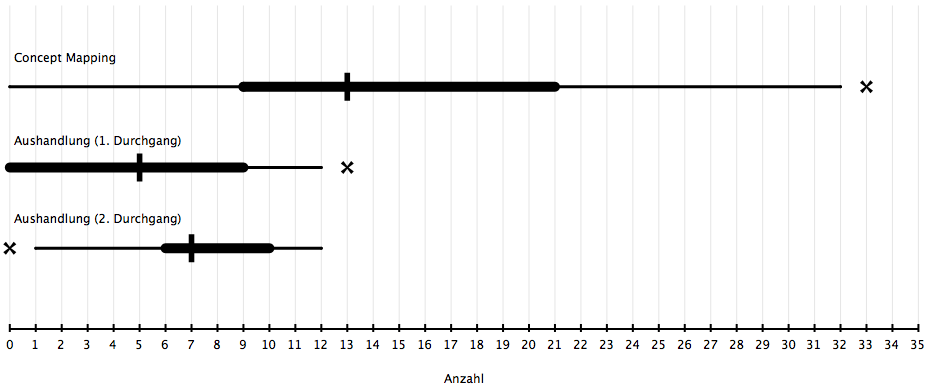
\includegraphics[width=15cm]{img/Evaluierung/elementUsageConnectorsOverview.png}
	\caption{Anzahl der verwendeten Verbindungen -- Übersicht}
	\label{fig:img_Evaluierung_elementUsageConnectorsOverview}
\end{figure}

Eine ähnliche Verteilung wie im Falle der Elemente ergibt sich bei Betrachtung der Anzahl der Verbindungen (siehe Abbildung \ref{fig:img_Evaluierung_elementUsageConnectorsOverview}). Auffällig ist jedoch die gegenüber Durchgang 2 des Aushandlungsblocks geringere Anzahl von Verbindungen in Durchgang 1 während sich die Anzahl der Blöcke zwischen den beiden Modellierungsdurchgängen umgekehrt verhält. Wie in der Überprüfung der Hypothese \ref{hyp:verbinder} in Abschnitt \ref{sub:herstellung_von_verbindern} bestätigt, ist dieses Phänomen auf die Fehlfunktionen und Instabilität der ursprünglichen Funktion zur Herstellung von Verbindungen zurückzuführen, die in Durchgang 1 ausschließlich zur Verfügung stand, während in Durchgang 2 (und auch im Block „Concept Mapping“) bereits die zusätzliche Funktion zur Verbindungsherstellung verfügbar war.

% subsubsection modellgröße (end)

\subsubsection{Vernetzungsgrad} % (fold)
\label{ssub:vernetzungsgrad}

Der Vernetzungsgrad der Modelle („Connectedness“) wurde bereits zur Überprüfung der Hypothese \ref{hyp:verbinder} in Abschnitt \ref{sub:herstellung_von_verbindern} betrachtet, ist jedoch eine Eigenschaft der erstellten Modelle an sich und wird hier deshalb nochmals als deskriptiver Parameter beschrieben.

\begin{figure}[htbp]
	\centering
		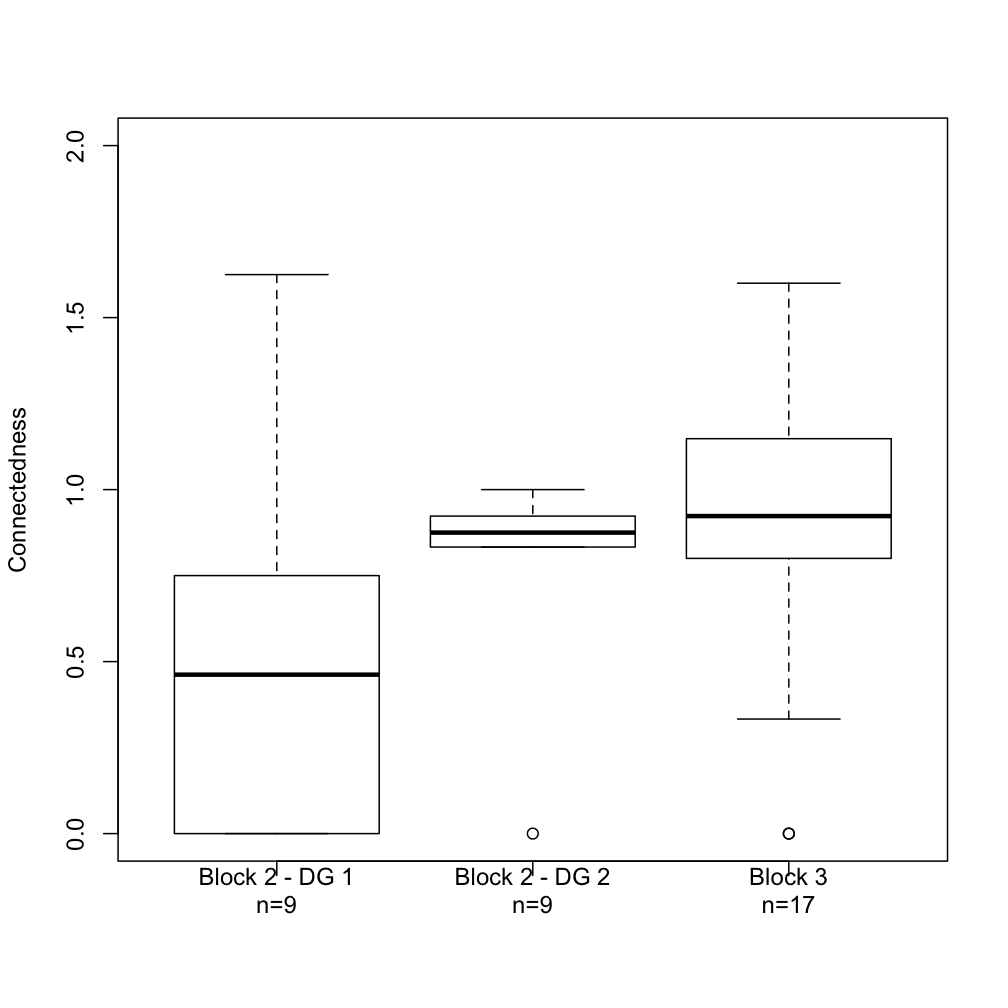
\includegraphics[width=10cm]{img/Evaluierung/connectednessOverview.png}
	\caption{Vernetzungsgrad (Verbindungen / Blöcke) -- Übersicht}
	\label{fig:img_Evaluierung_connectednessOverview}
\end{figure}

Abbildung \ref{fig:img_Evaluierung_connectednessOverview} zeigt die Verteilung des Verhältnisses der Anzahl von Verbindungen und Blöcken in den Modellierungsblöcken 2 und 3. Zu erkennen ist der oben und in Abschnitt \ref{sub:herstellung_von_verbindern} bereits beschriebene geringere Vernetzungsgrad im ersten Durchgang von Modellierungsblock 2 der auf die Instabilität und schwierige Verwendbarkeit der ursprünglichen Funktion zur Herstellung von Verbindungen zurückzuführen ist.

Seit der Verfügbarkeit der neuen Funktion zur Herstellung von Verbindungen (also im zweiten Teil von Block 2 sowie in den Blöcken 3, 4 und 5) liegt der Vernetzungsgrad im Mittel immer um 1, wobei in den letzten Blöcken (4 und 5) tendenziell noch höhere Vernetzungsgrade auftreten (Bock 4 im Mittel $1,32$, Block 5 im Mittel XY). Im Falle von Block 4 kann dies teilweise auf die Aufgabenstellungen zurückgeführt werden, die zum Teil starken Fokus auf die Repräsentation von Beziehungen legte (maximaler Vernetzungsgrad in einem Durchgang: $24/8=3$). Bei beiden Blöcken wurden außerdem weitere Stabilisrierungsmaßnahmen in der Interaktions-Erkennungsleistung des Systems vorgenommen, weshalb der gestiegene Vernetzungsgrad zum Teil auch auf die einfachere Herstellbarkeit von Verbindungen zurückgeführt werden kann (siehe wiederum \ref{sub:herstellung_von_verbindern}).

% subsubsection  (end)
% subsection m_durchführung (end)
% section untersuchungsdesign (end)

\section{Ergebnisse} % (fold)
\label{sec:m_ergebnisse}

\subsection{Keine semantische Einschränkung der Externalisierung} % (fold)
\label{sub:keine_semantische_einschränkung_der_externalisierung}

Gegenstand der hier beschriebenen Untersuchung Hypothese \ref{hyp:keine_einschränkung} („Das Werkzeug schränkt Benutzer semantisch nicht bei der Externalisierung ihrer mentalen Modelle ein.“). Als Grundlage dieser Untersuchung dienen die Ergebnisse der Modellierungsblöcke 2 bis 5, da in diesen die den einzelnen Modellelementen zugewiesene Semantik explizit untersucht wurde. Die Daten hinsichtlich der empfundenen Einschränkung bei der Modellbildung stammen aus der Befragung, die im Rahmen des Modellierungsblocks 4 durchgeführt wurde. Zusätzlich wurde das Videomaterial aller fünf Modellierungsblöcke zur Auswertung herangezogen.

\subsubsection{Auswertung} % (fold)

Die „Nicht-Einschränkung“ der Benutzer bei der Externalisierung kann wie in Abschnitt \ref{ssub:keine_semantische_einschränkung_der_externalisierung} beschrieben anhand des Modellierungsverhaltens der Benutzer beurteilt werden. Von Interesse ist hier die Zuweisung von Bedeutung (also semantischer Information) zu den (semantisch nicht vorbelegten) Modellierungselementen. Davon stehen grundsätzlich drei Arten von Blöcken („rot“, „gelb“, „blau“) sowie drei Arten von Verbindern („ungerichtet“, „gerichtet“, „bidirektional“). Erhoben wurde, wie viele Elemente im Verlauf der Modellierung mit Bedeutung belegt wurden, ob die Teilnehmenden mehr als die zur Verfügung stehenden Elemente benötigt hätten und ob ein Element im Modellierungsverlauf mit mehr als einer Bedeutung belegt wurde. 

Zu beachten ist hier, das die Bedeutungsbelegung immer Ergebnis eines Aushandlungsprozesses zwischen mindestens zwei Beteiligten ist. Aus dieser Teiluntersuchung kann also kein Rückschluss auf die individuell empfundene Einschränkung der Externalisierung getroffen werden. Nachdem der Prozess der Bedeutungsfestlegung aber inhärenter Bestandteil der kooperativen Modellbildung ist und die Zielsetzung derselben die Herstellung eines gemeinsamen Verständnisses ist, ist dies im Falle einer tatsächlich kooperativ vorgenommenen Festlegung der Bedeutung nicht als Einschränkung zu sehen. Eine individuell als einschränkend wahrgenommene Situation kann vielmehr dann auftreten, wenn die Bedeutungsfestlegung nicht kooperativ durchgeführt wurde, sondern die Bedeutungen von einem Teilnehmenden vorgegeben wurde. Diese Fälle sind in der folgenden Tabelle separat ausgeführt. Die individuell empfundene Einschränkung wurde außerdem im zweiten Teil der hier beschriebenen Untersuchung mittels einem auf dem \gls{PMS} basierenden Fragebogen sowie einer Auswertung der offenen Fragen zur Eignung des Werkzeugs zur Modellbildung erhoben. 

In der folgenden Tabelle\footnote{MB \ldots Modellierungsblock, x E.\ldots x Elemente mit Bedeutung belegt, x V. \ldots x Arten von Verbindungen verwendet} ist für jeden Modellierungsblock ausgeführt, in wie vielen Fällen eine bestimmte Anzahl von Blöcken mit Bedeutung belegt wurde und wie viele Arten von Verbindern benutzt wurden. Unterschiedliche Bedeutungen auf unterschiedlichen Modellebenen (also in eingebetteten Teilmodellen) wurden ohne separaten Unterscheidung mitgezählt.

\todo
\begin{tabular}{| p{1 cm} || p{1cm} | p{1cm} | p{1cm} | p{1.2cm} || p{1cm} | p{1cm} | p{1cm} | p{1.2cm} |}
  \hline
   MB & 1 E. & 2 E. & 3 E. & 4+ E. & 1 V. & 2 V. & 3 V. & 4+ V. \\ \hline
   2 - 1 & 0 & 2 &  9 & 0 & 4 & 1 & 0 & 0 \\ 
   2 - 2 & 1 & 0 &  8 & 0 & 6 & 1 & 0 & 1 \\ 
   3     & 0 & 3 & 14 & 0 & 6 & 4 & 0 & 6 \\ 
   4     & 0 & 2 &  7 & 2 & 3 & 4 & 2 & 1 \\ 
   5     & & & & & & & & \\ \hline
   Ges.  & & & & & & & & \\ \hline
\end{tabular} 
 
In jenen beiden Fällen in Modellierungsblock 5, in denen 4 oder mehr bedeutungstragende Elemente verwendet wurden, wurden im ersten Fall 6 und im zweiten Fall 7 Elementtypen festgelegt. Beide Modelle enthielten jedoch ineinander verschachtelte Teilmodelle, von denen keines mehr als drei Typen beinhaltete. Jene Fälle, in denen 4 oder mehr verschiedene Arten von Verbindern verwendet wurden, kamen durch den Einsatz benannter Verbinder zustande, mittels derer die Bedeutung der Verbindungen beliebig differenziert werden kann.

Im zweiten Teil der Untersuchung zu dieser Hypothese wurden qualitativ einerseits die expliziten Aussagen der Teilnehmenden ($n_{ges}=147$) hinsichtlich einer eventuellen einschränkenden Wirkung des Werkzeugs gesammelt, andererseits wurden die Videoaufnahmen der Werkzeuganwendungen diesbezüglich ausgewertet. Folgende Punkte mit einschränkender Wirkung konnten hier identifiziert werden (in Klammern jeweils die Quellen sowie die Anzahl des Auftretens der jeweiligen Aussage):
\begin{itemize}
	\item Unterschiedliche Farben von Verbindern wären wünschenswert (Befragung in Block 4, $n=2$)
	\item Drei unterschiedliche Elementtypen sind zu wenig (verbales Feedback von Personen mit praktischen Prozessmodellierungskenntnissen\footnote{Nach diesen Kenntnissen wurde im Rahmen einer Selbsteinschätzung explizit gefragt} in den Blöcken 2 und 4 sowie in nicht formal dokumentieren Modellierungssitzungen mit Prozessmodellierungsexperten\footnote{jeweils nach Eigendeklaration bzw. aus dem professionellen Umfeld der Personen geschlossen} im Rahmen von Demonstrationen auf mehreren Konferenzen, $n=7$)
	\item Dezidierte Elemente zur Modellierung von Verzweigungen und Parallelisierungen im Kontrollfluss wären wünschenswert (verbales Feedback von Personen mit Prozessmodellierungskenntnissen in den Blöcken 2 und 4 sowie in nicht formal dokumentieren Modellierungssitzungen mit Prozessmodellierungsexperten im Rahmen von Demonstrationen auf mehreren Konferenzen, $n=5$)
	\item Selbst festlegbare Formen, Farben und/oder Größen von Modellelementen wären wünschenswert (verbales Feedback von Personen in Block 4 sowie in nicht formal dokumentieren Modellierungssitzungen mit  Strukturaufstellungsexperten\footnote{das Werkzeug scheint sich zur Unterstützung von Strukturaufstellungen \citep{Sparrer02} zu eignen, dies wurde jedoch im Rahmen dieser Arbeit weder als Anwendungsfall vorgesehen, noch formal getestet} im Rahmen von Demonstrationen auf mehreren Konferenzen, $n=3$)
\end{itemize}

Explizite Aussagen zu einer dezidiert „nicht-einschränkenden“ Wirkung bzw. der semantischen Offenheit des Werkzeugs konnten nur in Fällen identifiziert werden, in denen explizit nach diesem Aspekt gefragt wurde. In diesen Fällen wurde der Umfang der Ausdrucksmöglichkeiten durchwegs als ausreichend erachtet. Personen ohne Vorkenntnisse in der Prozessmodellierung empfanden die Anzahl der zur Verfügung stehenden Elemente im Allgemeinen als ausreichend, jene Fälle in denen dies nicht der Fall war, sind oben dokumentiert.

Lediglich in einem\footnote{in Modellierungsblock 3} der dokumentierten Fälle ($n=65$) waren die Teilnehmenden mit der eigenständigen Wahl der Bedeutung der Elementtypen überfordert und begannen nicht eigenständig zu modellieren. Erst nach einer teilweisen bzw. beispielhaften Vorgabe von 2 Elementtypen durch den Untersuchungsleiter konnten die Teilnehmenden die Modellierung selbständig fortführen. 

Vergleichend ist festzustellen, dass beim Einsatz der Werkzeugs „CMapTools“, das die Anzahl der Elementtypen nicht einschränkt, in Modellierungsblock 5 ($n=12$) zwischen 1 und 8 Elementtypen verwendet wurden, wobei der Median bei 3 liegt. In je einem Fall wurden 1, 7 und 8 Elementtypen verwendet, in zwei Fällen wurden 3 Elementtypen eingesetzt, in drei Fällen kamen 4 Typen und in vier Fällen 2 Elementtypen zum Einsatz.

\subsubsection{Diskussion} % (fold)

Betrachtet man die Ergebnisse der quantitativen Auswertung der Einsätze des Werkzeugs in den Modellierungsblöcken 2 bis 5, so scheint die gegebene Ausdrucksstärke für die Modellierung weitgehend ausreichend zu sein. Dieser Eindruck relativiert sich bei einer vergleichenden Betrachtung mit einem computerbasierten, semantisch vollständig offenen Werkzeug sowie bei Betrachtung der qualitativen Auswertung der Benutzeraussagen sowie der Videoaufnahmen. 

In der vergleichend durchgeführten Studie in Modellierungsblock 5 zeigt sich, dass bei keiner Einschränkung der Anzahl der Modellelementtypen in mehr als der Hälfte der Fälle mehr als die im hier betrachteten Werkzeug zur Verfügung stehenden drei Elementtypen verwendet werden. Dies scheint darauf hinzudeuten, dass sich die Teilnehmenden an der beschränkten Anzahl der zur Verfügung stehenden Elemente orientieren, auch wenn dies -- wie aus den Aussagen der Teilnehmenden bei der ex-post-Befragung ersichtlich -- bis auf einige Ausnahmen nicht als Einschränkung wahrgenommen wird.

Aus den qualitativen Rückmeldungen zur Modellierung zeigt sich außerdem, dass Personen, die in ihrer täglichen Arbeit aktiv mit Prozessmodellierung beschäftigt sind, bei Aufgabenstellungen, die aufgrund ihrer Fragestellung zu Ablaufbeschreibungen führen, eher die Verwendung von mehr als drei Elementtypen bevorzugen würden. Personen, denen Prozessmodellierung fremd ist oder deren Erfahrung damit sich auf eine einmalige, länger zurückliegende Ausbildung beschränkt, konnten ihre Modelle zu ablauforientierten Fragestellungen ohne Ausnahme mit maximal drei Elementtypen abbilden. Bei nicht ablauforientierten Fragestellungen ist diese Unterscheidung nicht zu beobachten.

In Einzelfällen wurden außerdem weitere Wünsche zur Steigerung der Ausdrucksmöglichkeiten im Modell geäußert. Neben dem Wunsch nach unterschiedlich einfärbbaren Verbindungen zwischen Elementen wurde vor allem der Wunsch nach der Verwendung beliebiger Gegenstände als Modellelemente mehrfach geäußert, was das Einbringen von Repräsentation aus der alltäglichen Arbeitspraxis anstelle der abstakten Modellelemente erlauben würde.

Unter Berücksichtigung dieser Einschränkungen kann die hier betrachtete Hypothese mit Vorbehalten bestätigt werden. Tatsächlich scheint das Werkzeug bis auf wenige Ausnahmen nicht als semantisch einschränkend wahrgenommen zu werden, die Ergebnisse der vergleichenden Studie weisen aber auf eine einschränkende Wirkung durch die auf drei beschränkte Anzahl von Elementtypen hin.

\subsubsection{Ergebnis} % (fold)

\textbf{Die Hypothese \ref{hyp:keine_einschränkung} kann in der Untersuchung mit Vorbehalten angenommen werden.} Die Verwendung des Werkzeugs zur Modellierung scheint (bis auf wenige Ausnahmen) nicht als semantisch einschränkend wahrgenommen zu werden. Die vergleichende Studie aus Modellierungsblock 5 deutet allerdings auf eine einschränkende Wirkung durch die auf drei beschränkte Anzahl von Elementtypen hin.

% subsection keine_semantische_einschränkung_der_externalisierung (end)

\subsection{Repräsentation beliebig umfangreicher Modelle} % (fold)
\label{sub:repräsentation_beliebig_komplexer_modelle}

Gegenstand der hier beschriebenen Untersuchung Hypothese \ref{hyp:beliebige_komplexität} („Das Werkzeug ermöglicht die Repräsentation beliebig umfangreicher Modelle.“). Als Grundlage dieser Untersuchung dienen die Ergebnisse der Modellbildung in Modellierungsblock 3 und 5 sowie die Befragungen in den Modellierungsblöcken 1 bis 5.

\subsubsection{Auswertung} % (fold)

Von Interesse ist bei der Prüfung dieser Hypothese der Vergleich des Umfangs von Modellen, die mit dem hier vorgestellten Werkzeug erstellt wurden, mit Modellen, die mit einem bezogen auf die Größe der Arbeitsfläche unbeschränkten Werkzeug erstellt wurden. Diese vergleichende Studie wurde im Rahmen der Untersuchungen in Block 5 durchgeführt. Als Metrik zum Vergleich der Modellgrößen wurde die Anzahl der Modellelemente verwendet. Abbildung \ref{fig:img_Evaluierung_ElementeConceptMapping2} zeigt eine Gegenüberstellung der Modellgrößen bei Verwendung der „CMapTools“ als die Größe nicht beschränkendes Werkzeug und dem hier vorgestellten System\footnote{In allen Boxplots gilt folgende Notation: 
\begin{itemize}
	\item breite horizontale Linie: Bereich zwischen 25\%- und 75\%-Quantil
	\item breite vertikale Linie: Median
	\item linke schmale Linie: Bereich zwischen 2,5\%- und 25\%-Quantil
	\item rechte schmale Linie: Bereich zwischen 75\%- und 97,5\%-Quantil
	\item Kreuze: Ausreißer (außerhalb 2,5\%- und 97,5\%-Quantil)
\end{itemize}
}.

\begin{figure}[htbp]
	\centering
		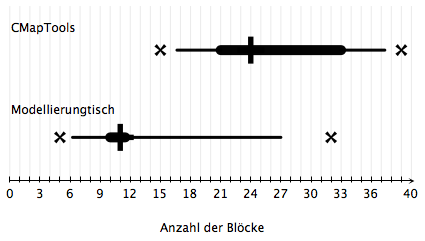
\includegraphics[width=10cm]{img/Evaluierung/ElementeConceptMapping2.png}
	\caption{Gegenüberstellung der Modellgrößen in Modellierungsblock 5}
	\label{fig:img_Evaluierung_ElementeConceptMapping2}
\end{figure}

Die Betrachtung der Ergebnisse zeigt, dass die Modelle, die mittels der „CMapTools“ erstellt wurden ($M=25.92, SD=7.04, N=12$), signifikant umfangreicher waren (einseitiger t-Test für zwei ungepaarte Stichproben ungleicher Varianz $t(21)=4.74, p<=0.001$), als jene Modelle, die mittels dem hier vorgestellten System erstellt wurden ($M=12.18, SD=6.84, N=11$).

In den Modellierungsblöcken 3 und 5 wurden insgesamt 30 Modellierungsdurchgänge durchgeführt, deren Ergebnis aufgrund der Aufgabenstellung bei detaillierte Modellierung mehr als 15 Modellierungselement enthalten müsste (siehe vergleichende Ergebnisse aus Block 5). In insgesamt 7 Fällen wurden mehr als 15 Elemente verwendet ($15<x<=20: 1, 20<x<=25: 2, 25<x<=30: 2, x>30: 2$), der Median der Anzahl der Elemente liegt bei 11 ($M=14.68, SD=7.90, N=30$). Die Möglichkeit der Einbettung von Teilmodellen wurde insgesamt in 8 Modellierungsdurchgängen genutzt, davon war in drei Fällen die Gesamtanzahl der Elemente geringer als 15 (womit eine rein semantische Strukturierung vorliegt und keine Steigerung der Modellumfangs vorgenommen wurde).

Neben der vergleichenden Studie wurde in allen Modellierungsblöcken der subjektive Eindruck der Teilnehmenden nach einer etwaig einschränkenden Wirkung hinsichtlich des Umfangs der Modelle gefragt ($n_{ges}=147$). Insgesamt 43 Teilnehmende empfanden die Modellierungsoberfläche als zu klein um die gewünschten Sachverhalte abzubilden. Von insgesamt 9 Teilnehmenden wurde explizit der Wunsch nach kleineren Elementen geäußert, um umfangreichere Modelle abbilden zu können. Von 23 Teilnehmenden wurde die Visualisierung der Verbindungen kritisiert („unübersichtlich“, „nur eine Verbindung zwischen zwei Blöcken möglich“), was dazu geführt hätte, dass die Modelle nicht wie ursprünglich intendiert aussähen.

\subsubsection{Diskussion} % (fold)

Sowohl die quantitativen Ergebnisse auf Modellierungsblock 5 als auch die qualitativen Ergebnisse weisen darauf hin, dass die physische Realisierung der Modells, die mit eine Beschränkung der Modellierungsoberfläche einher geht, die Abbildung beliebig umfangreicher Modelle nicht erlaubt.

Bei der Gegenüberstellung des quantitativen Teils der Studie mit den qualitativen Aussagen der Teilnehmenden fällt auf, dass -- wie bereits bei der Diskussion der Hypothese \ref{hyp:keine_einschränkung} in Abschnitt \ref{sub:keine_semantische_einschränkung_der_externalisierung} -- die subjektive Wahrnehmung der Einschränkung weniger stark ausgeprägt ist als die vermutete tatsächliche Einschränkung, auf die aufgrund der quantitativen Daten geschlossen werden kann. Tatsächlich ist jedoch der Anteil der Teilnehmer, die das Modell nicht so umfangreich wie intendiert abbilden konnten, höher als jener die sich in der semantischen Ausdrucksstärke eingeschränkt fühlten.

Aus den qualitativen Aussagen ist zu erkennen, das der vorrangige Grund der Beschränkung des Modellumfangs die eingeschränkte Größe der Modellierungsoberfläche ist. Die Möglichkeit zur Einbettung von Teilmodellen zur Steigerung des Umfangs wurde nur in einem Sechstel der Fälle verwendet, was darauf hindeutet, dass diese Funktion keinen Ersatz für eine unbeschränkt große Modellierungsoberfläche (auf einer Abstraktionsebene) darstellt.

Insgesamt kann aufgrund der Ergebnisse der Untersuchung die Hypothese \ref{hyp:beliebige_komplexität} nicht bestätigt werden.

\subsubsection{Ergebnis} % (fold)

\textbf{Die Hypothese \ref{hyp:beliebige_komplexität} kann in der Untersuchung nicht bestätigt werden.} Modelle, die mit dem hier vorgestellten Werkzeug erstellt wurden, weisen bei identischer Aufgabenstellung einen signifikant geringeren Umfang auf als Modelle, die mit einem Werkzeug mit nicht beschränkter Arbeitsfläche erstellt wurden. Auch das qualitative Feedback der Benutzer deutet darauf hin, dass eine vollständige Abbildung eines Modells (und damit die Erstellung eines Modells mit größerem Umfang) nicht bzw. nur umständlich möglich ist.

% subsection repräsentation_beliebig_komplexer_modelle (end)

% subsection abstimmung_individueller_modelle (end)

\subsection{Wirkung auf die Kooperation bei der Modellerstellung} % (fold)
\label{sub:wirkung_auf_die_kooperation_bei_der_modellerstellung}

\todo Zeitverteilung aus Block 5 fehlt noch

\subsubsection{Auswertung} % (fold)

\subsubsection{Diskussion} % (fold)

\subsubsection{Ergebnis} % (fold)

% subsection wirkung_auf_die_kooperation_bei_der_modellerstellung (end)

\subsection{Abbildung von Zusammenhängen ohne Verbinder} % (fold)
\label{sub:abbildung_von_zusammenhängen_ohne_verbinder}

Gegenstand der hier beschriebenen Untersuchung Hypothese \ref{hyp:keine_verbinder} („Zur Abbildung von Zusammenhängen ist die Verwendung von Verbindern nicht notwendig.“). Als Grundlage dieser Untersuchung dienen die Befragungen sowie die Videoaufnahmen der Modellierungsblöcke 1 bis 5.

\subsubsection{Auswertung} % (fold)

In insgesamt 18 von den in allen 5 Modellierungsblöcken 64 erstellten Modellen (für eine detaillierte Aufstellung siehe Abschnitt \ref{sub:repräsentation_diagrammatischer_modelle}) wurden keine Verbinder zur Darstellung von Zusammenhängen zwischen Elementen verwendet. Von diesen 18 Modellen wurden 9 Modelle (in den Modellierungsblöcken 2 und 3) während der Modellierung von allen Beteiligten kommunikativ interpretiert. Die Teilnehmenden wurden unmittelbar nach Abschluss der Modellbildung über ihre subjektive Wahrnehmung der Übereinstimmung des Verständnisses über den abgebildeten Sachverhalt befragt. Alle Teilnehmer ($n_{ges}=21$) gaben an, subjektiv ein gemeinsames Verständnis erreicht zu haben. Diese Angaben decken sich mit den Auswertungen der Modellierungsverläufe in diesen Durchgängen, in denen in 3 von 9 Fällen während der Modellierung der Eindruck entstand, dass Teile der Modelle unterschiedlich interpretiert wurden. Diese unterschiedlichen Interpretationen wurden jedoch in allen Fällen im weiteren Verlauf der Modellierung erkannt und so abgestimmt, das ein übereinstimmendes Verständnis hergestellt werden konnte.

Jene 9 Modelle, die in Modellierungsblock 1 erstellt wurden, wurden von Dritten interpretiert. Die Interpretation wurde dabei den ursprünglichen Modellerstellern rückgespiegelt, die wiederum zu beurteilen hatten, ob die Interpretation den ursprünglich repräsentierten Sachverhalt korrekt wiedergibt. Dies war in allen 9 Modellierungsdurchgängen der Fall.

Die übrigen 46 Modelle, in denen Verbinder verwendet wurden, wurden einer nachgelagerten Interpretation durch den Leiter der Studiendurchführung\footnote{dem Verfasser dieser Arbeit} unterzogen, der an der Durchführung von 17 Modellierungsdurchgängen als Untersuchungsleiter beteiligt war (die übrigen 29 Modellierungsdurchgänge wurden im Rahmen von Diplomarbeiten erfasst, wobei die jeweiligen Diplomanden als Untersuchungsleiter auftraten). Bei dieser Interpretation wurden im ersten Schritt für jedes Modell die verwendeten Verbinder entfernt und versucht, den Modellinhalt zu interpretieren. In einem zweiten Schritt wurden die Verbinder wieder eingeblendet und die Interpretation mit dem nun vollständigen Modell verglichen. Dabei ergaben sich in 15 Fällen Unterschiede in der Interpretation, die ausschließlich auf die Verwendung von Verbindern zurückzuführen war. In den übrigen 36 Fällen explizierten bzw. bestätigten die erstellten Verbindungen die durch die räumliche Anordnung der Modellierungselemente implizit ausgedrückten Zusammenhänge. Dabei ist zu anzuführen, dass in 13 der insgesamt 46 Modelle benannte Verbinder verwendet wurden (die übrigen 33 Modelle enthielten lediglich unbenannte Verbinder). Von diesen 13 Modellen konnten 4 auch ohne die Darstellung der Verbinder korrekt (im Sinne der obigen Ausführungen) interpretiert werden. Demnach führte die Entfernung der Verbinder in 6 der 33 Modelle mit unbenannten Verbindern zu unvollständigen bzw. fehlerhaften Interpretationen.

\subsubsection{Diskussion} % (fold)

Das weitgehende Fehlen von Verbindern ist in den ersten beiden Modellierungsblöcken sowie Teilen des Modellierungsblocks 3 auf die mangelhafte Funktion der Verbindungsherstellung durch Benutzer zurückzuführen (siehe Prüfung der Hypothese \ref{hyp:diagmodelle} in Abschnitt \ref{sub:repräsentation_diagrammatischer_modelle}). Trotzdem war es den Teilnehmenden möglich, ein gemeinsames Verständnis über die abgebildeten Zusammenhänge zu entwickeln. Auch bei der Interpretation durch Dritte, die am Entstehungsprozess des Modells nicht beteiligt waren, traten keine Missverständnisse auf. Dies gilt sowohl für ablauf-orientierte Modelle (in Modellierungsblock 1 und 2) als auch für Concept-Map-artige Modelle (in Modellierungsblock 3).

Insofern scheint die Hypothese bestätigt werden zu können. Diese Annahme ist insofern zu relativieren, als dass den Modellierungsblöcken 3, 4 und 5 insgesamt 15 Modellierungsdurchgänge identifiziert werden konnten, in denen die Verwendung von Verbindungen den Modellen Bedeutung hinzufügt, die ohne diese auch implizit nicht vorhanden gewesen wäre. Eine vorbehaltslose Annahme der Hypothese erschient deshalb nicht gerechtfertigt.

Hypothese \ref{hyp:keine_verbinder} kann unter Berücksichtigung der obigen Ausführungen damit nicht bestätigt werden. Während in vielen Fällen die ausschließliche räumliche Anordnung von Modellierungselementen ausreichend zu sein scheint, um die beabsichtigte Bedeutung zu kommunizieren, konnten Fälle identifiziert werden, in denen dies nicht möglich war.

\subsubsection{Ergebnis} % (fold)

\textbf{Die Hypothese \ref{hyp:keine_verbinder} kann auf Basis der Untersuchung nicht bestätigt werden.} Während zu Bildung eines einheitlichen Verständnisses in vielen Fällen die implizite Abbildung von Zusammenhängen durch räumliche Konfiguration der Modellierungselemente ausreichend erscheint, konnten Fälle identifiziert werden, in denen die explizite Repräsentation von Verbindern dem Modell Bedeutung hinzufügte, die ohne Darstellung derselben nicht kommunizierbar gewesen wäre.

% subsection abbildung_von_zusammenhängen_ohne_verbinder (end)
% section m_ergebnisse (end)

\section{Zusammenfassung} % (fold)
\label{sec:m_zusammenfassung}

In diesem Kapitel wurde die Evaluierung des Aspektes der Modellierung mit dem hier vorgestellten Werkzeug beschrieben. Die hier betrachteten Hypothesen beschäftigen sich mit dem Modellierungsergebnis ansich sowie dem Prozess der Modellerstellung. In Abgrenzung dazu wurde in Kapitel \ref{cha:eval_werkzeug} die Verwendung des Werkzeugs im Allgemeinen sowie dessen Verständlichkeit geprüft. Kapitel \ref{cha:eval_aw} beschäftigt sich hingegen mit der Rückwirkung der Modellierung bzw. der Modelle auf die eigentlichen Betrachtungsgegenstände (also etwa operative Arbeitsabläufe).

Im Rahmen dieses Kapitels wurden drei aus der Aufgabenstellung begründbare Hypothesen und eine explorativ während der Evaluierung gebildete Hypothese getestet. Die ersten beiden Hypothesen beschäftigen sich mit einer eventuell einschränkenden Wirkung des Werkzeugs auf die Modellbildung. Wie in den Anforderungen \ref{anf:nicht_vorgegebene_semantik_der_modellierungselemente} und \ref{anf:bearbeitung_von_beliebig_komplexen_modellen} formuliert, muss das Werkzeug zur Unterstützung von „Articulation Work“ einerseits semantische Offenheit bei der Modellierung bieten (d.h. die Modellierenden nicht bei der Abbildung der eigenen Konzeptualisierung des abzubildenden Sachverhaltes einschränken) und andererseits die Abbildung beliebig umfangreicher Modelle erlauben. 

Hypothese \ref{hyp:keine_einschränkung} („Semantische Offenheit“) konnte dabei insofern bestätigt werden, als dass die Teilnehmenden das Werkzeug nur in Einzelfällen als semantisch einschränkend empfanden. Der Vergleich mit einem semantisch vollständig offenen Werkzeug, dass die Anzahl der Elementtypen im Gegensatz zum vorliegenden Werkzeug nicht beschränkt, deutet jedoch darauf hin, dass in manchen Anwendungsfällen tatsächlich mehr als die drei im Werkzeug semantisch belegbaren Elementtypen zum Einsatz kommen sollten.  

Hypothese \ref{hyp:beliebige_komplexität} („Beliebiger Modellumfang“) konnte im Rahmen der Untersuchung nicht bestätigt werden. Die beschränkte Größe der Modellierungsoberfläche scheint einschränkend auf den Modellumfang zu wirken, die Möglichkeit der Einbettung von Teilmodellen ist dabei kein adäquater Ersatz. In einer vergleichenden Studie mit einem die Arbeitsfläche nicht beschränkenden Werkzeug wurden bei identischer Aufgabenstellung im Durchschnitt Modelle mit doppelten Umfang als auf dem hier vorgestellten Werkzeug erstellt. Auch die Rückmeldungen der Teilnehmenden deuten darauf hin, dass die Beschränkung der Modellierungsoberfläche in vielen Fällen als einschränkender Faktor wahrgenommen wird.

Hypothese \ref{hyp:stärkere_kooperation} untersucht, ob die Verwendung des Werkzeugs zu stärkerer Kooperation führt als die Verwendung eines bildschirmbasierten Werkzeugs. Diese Hypothese konnte im Rahmen der Untersuchung ... \todo

Die letzte in diesem Kapitel untersuchte Hypothese (Hypothese \ref{hyp:keine_verbinder}) betraf die explorativ gebildete Vermutung, dass zur Repräsentation von Zusammenhängen in Modellen die explizite Darstellung von Verbindern nicht notwendig wäre sondern die ausschließliche räumliche Konfiguration der Modellierungselemente zueinander ausreichen würde, um die Zusammenhänge erfassbar zu machen. Während dies im überwiegenden Teil der Anwendungsfälle möglich war, konnten Modelle identifiziert werden, in denen die Verbinder Information codierten, die rein durch die räumliche Anordnung der Modellelemente nicht ableitbar gewesen wäre (in etwa 25\% der Fälle). Hypothese  \ref{hyp:keine_verbinder} konnte im Rahmen der Untersuchung damit nicht bestätigt werden.

% section zusammenfassung (end)
% chapter eval_modell (end)